
\documentclass[a4paper]{article}

\usepackage{graphicx}
\usepackage{listings}
\usepackage{indentfirst}
\usepackage{float}
%\usepackage[T1]{fontenc}                % F�r svenska bokst�ver
%\usepackage[swedish]{babel}             % F�r svensk avstavning och svenska
                                        % rubriker (t ex "inneh�llsf�rteckning)
\title{Programming Project, C++ Programming}
\author{Tim Dolck dat11tdo@student.lu.se \\ 
  Julian Kron\'{e} dat11jkr@student.lu.se \\
Computer science, LTH}
%\date{}           % Blir dagens datum om det utel�mnas

\begin{document}
\lstset{language=SQL}

\maketitle
\newpage
\section{Introduction}
\section{Requirements}
\subsection{General Requirements}
The system consists of a server that handles a database containing newsgroups and articles and a
client that accepts commands from the user and communicates with the server. 
Several clients may be connected to the server simultaneously.
The following tasks can be performed:
\begin{itemize}
  \item List newsgroups.
  \item Create and delete newsgroups.
  \item List articles in a newsgroup.
  \item Read, write and delete articles in a newsgroup.
\end{itemize}
The system keeps track of the title and the author of each article. 
The communication between the server and the client follows the predefined messaging protocol.
There are no security requirements on the system. For instance, any user can delete news-
groups and articles, even if he or she is not the creator.

\subsection{Server Requirements}
There are two versions of the server: 
\begin{enumerate}
  \item A server that uses a database stored in primary memory.
  \item A server that uses a database stored on disk.
\end{enumerate}
The in-memory version of the server starts from scratch each time it is invoked and builds
the database in primary memory.

The disk version of the database remembers the database between invocations. Changes to
the database are immediately reflected on disk.

Each newsgroup has a unique name. A newsgroup also has a unique identification number,
greater than zero. Identification numbers may not be reused.

Each article has a title, an author and an article text. The article names need not be unique.
An article also has an identification number, which must be unique in the newsgroup.
Identification numbers may not be reused.

Listings of newsgroups and articles are in chronological order, with the oldest item first.

There are no limitations on the number of newsgroups or the number of articles in a
newsgroup.

There are no limitations on the length of newsgroup titles, article titles, author names or
article texts.

If a client misbehaves, for example by not following the messaging protocol, it is immediately
disconnected by the server.

The server tries to handle all errors. If it cannot recover from an error, it terminates with an
informative error message.

\subsection{Client Requirements}
The clients reads commands from the keyboard, communicates with the server and presents
the replies from the server on the terminal.

The client is easy to use and contains informative help texts. No manual is necessary to use
the client program.

The client tries to handle all errors. If it cannot recover from an error, it terminates with an
informative error message



\section{Outline}
\section{Model}
\section{System description}
\subsection{Uml}

\subsection{Classes}

\section{Conclusion}

An overview of the program design can be seen in figure~\ref{model}.

\begin{figure}[H]
  \centering
%  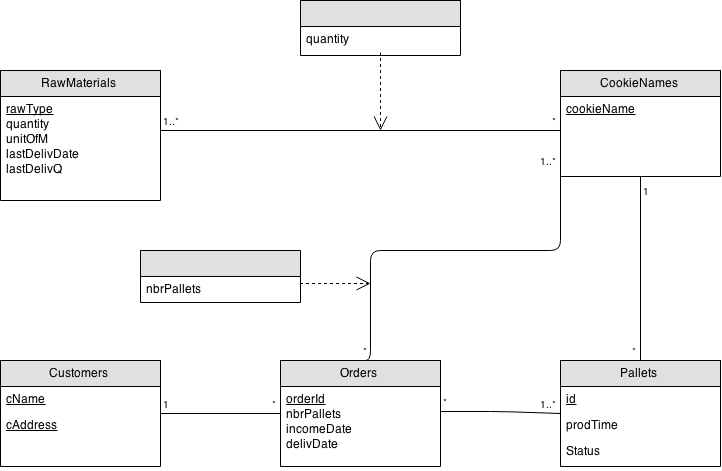
\includegraphics[width=\textwidth]{cookies.png}
  \caption{An UML diagram illustrating the database design.}
  \label{model}
\end{figure}

\end{document}                 % The input file ends with this command.
